\section{Theorie}
\label{sec:Theorie}

Ziel des Versuches ist die Bestimmung der effektiven Masse der Elektronen in Gallium-Arsenid mittels des Faraday-Effekts.

\subsection{Struktur und Klassifizierung von Festkörpern}
Aufgrund ihres periodischen Aufbaus besitzen kristalline Festkörper wie Gallium-Arsenid eine sogenannte Bandstruktur, die typischerweise als Energie $E$ in Abhängigkeit vom Impuls $k$ darstellt wird.
In Abbildung \ref{fig:magnesium}
findet sich beispielhaft die Struktur von Magnesium im Ortsraum. Die verschiedenen quantisierten Energieniveaus führen dazu, dass sich diese Bänder ausbilden. Von Interesse ist dabei das letzt besetzte und erste unbesetzte Band.
Bei dem letzten (vollständig) besetzten Band wird vom Valenzband gesprochen, das erste unbesetzte Band ist das Leitungsband. Die Lage dieser Bänder zueinander zusammen mit der Fermi-Energie, also der höchsten Energie der Elektronen
beim absoluten Nullpunkt, bestimmen, ob es sich um ein Metall, einen Halbleiter oder einen Isolator handelt.

\begin{figure}[H]
    \centering
    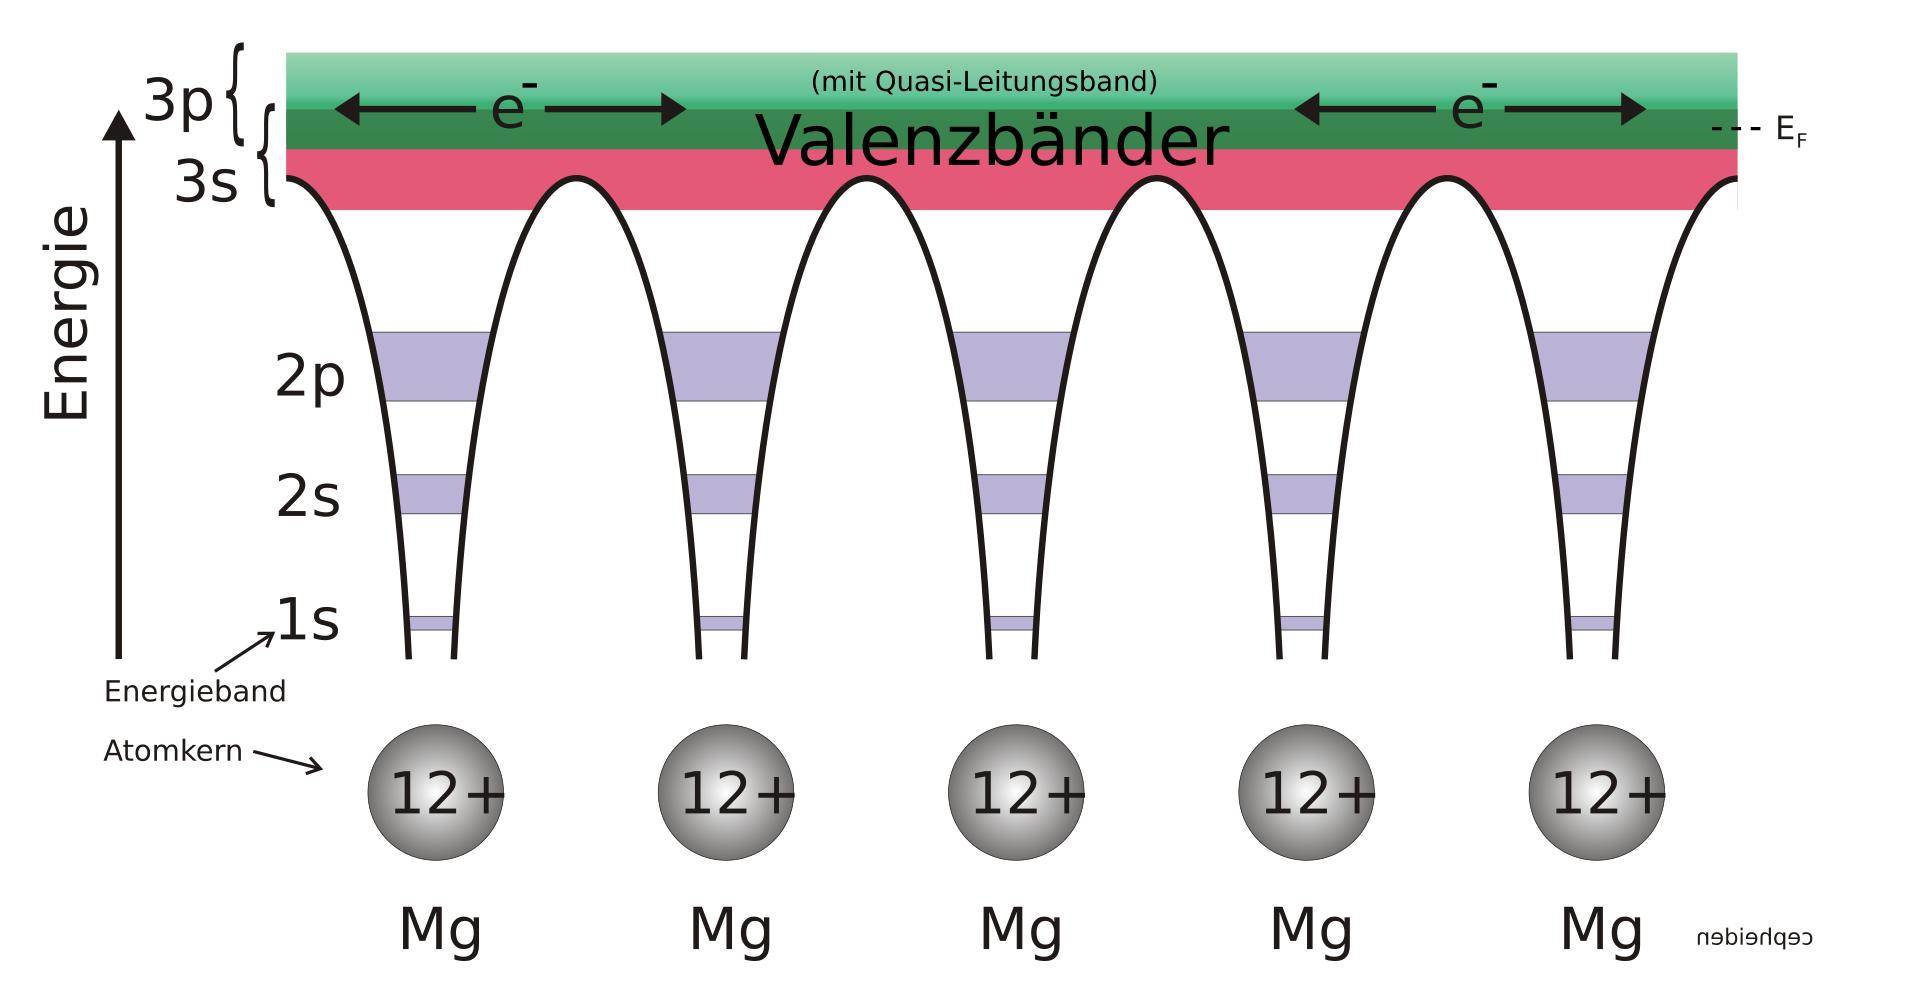
\includegraphics[width=\textwidth]{Bilder/Bändermodell-Potentialtöpfe-Mg.svg.png}
    \caption{Bändermodell von Magnesium im Ortsraum. \cite{magnesium} }
    \label{fig:magnesium}
\end{figure}
Im Fall von Metallen, zum Beispiel dem Magnesium in Abbildung \ref{fig:magnesium},
überlappen sich das Valenz- und das Leitungsband und die Fermi-Energie liegt in diesem Überlapp. \\
Im Fall von Halbleitern und Isolatoren überlappen sich das Valenz- und Leitungsband nicht, es gibt also eine Bandlücke, und die Fermi-Energie liegt in dieser Lücke. Ist die Bandlücke kleiner als $\qty{3}{\electronvolt}$, wird von von Halbleitern gesprochen,
Bandlücken größer als das sind Isolatoren. \\
Halbleiter können dotiert werden, was bedeutet, dass gezielt Verunreinigungen in den Kristall eingebracht werden, die je nach Bedarf mehr oder weniger Elektronen besitzen.
Ein Kristall aus der vierten Hauptgruppe, z.B. Silizium, was ebenfalls ein Halbleiter ist, kann mit Stoffen aus der dritten Hauptgruppe p-dotiert werden, was bedeutet, dass die Verunreinigungen sogenannte Löcher
in den Kristall bringen, die als Ladungsträger für die Leitung fungieren. Stoffe aus der fünften Hauptgruppe würden ein weiteres Elektron einfügen, der Kristall wäre also n-dotiert, ein quasi-freies Elektron kann geleitet werden\\
Die Energieniveaus von diesen Akzeptoren bzw. Donatoren liegen entsprechend etwas überhalb des Valenzbandes bzw. unterhalb des Leitungsbandes, sie können also sehr leicht Elektronen aus dem Valenzband aufnehmen bzw. an das Leitungsband abgeben.

\begin{figure}[H]
    \centering
    \includegraphics[width=\textwidth]{Bilder/bänder.png}
    \caption{Bändermodell im Ortsraum, sehr vereinfacht. \cite{magnesium}}
    \label{fig:bänder}
\end{figure}

\subsection{Effektive Masse}
Die Elektronen im Festkörper spüren ständig das Potential der Atomrümpfe, was schließlich auch zur Bandstruktur führt. Um die Elektronen wie quasi-freie Teilchen zu behandeln, wird die sogenannte effektive Masse eingeführt,
mit der die Bewegungsgleichungen ihre Gültigkeit behalten. Die effektive Masse lautet
\begin{equation}
    m^{*} = \hbar^2 \left( \frac{\text{d}E}{\text{d}k^2} \right) ^{-1}.
    \label{eq:effektive_masse}
\end{equation}
Im Banddiagramm entspricht sie also dem Inversen der Krümmung, also dem Krümmungsradius des Bandes. In annähernd parabolischen Bändern ist sie also konstant.\\
In der Struktur von Gallium-Arsenid in \ref{fig:gaas} erkennt man die parabolische Struktur sowie die Bandlücke von $\qty{1.42}{\electronvolt}$.
\begin{figure}[H]
    \centering
    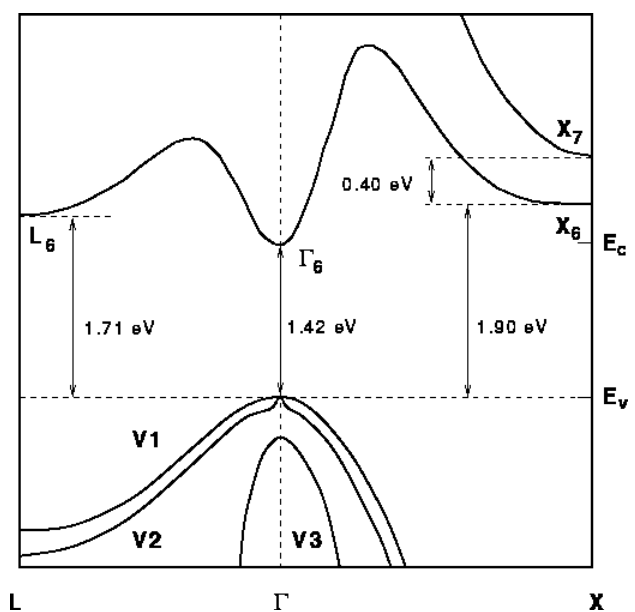
\includegraphics[width=\textwidth]{Bilder/gaas.png}
    \caption{Bandstruktur von Gallium-Arsenid. \cite{gaas}}
    \label{fig:gaas}
\end{figure}


\subsection{Faraday Effekt}
Licht hat eine Polarisation, die als die Schwingungsrichtung des elektrischen Anteils der elektromagnetischen Welle definiert wird. Diese Polarisation kann senkrecht oder parallel zu einer festgesetzten Fläche,
z.B. einem flachen Kristall, verlaufen, wie in \autoref{figf:aradayeffekt}
erkennbar. Ebenso gibt es zirkulare Polarisation, bei der die Polarisationsebene sich dreht. Zirkulare Polarisation kann über zwei lineare Polarisationen beschrieben werden, umgekehrt kann lineare Polarisation über zwei zirkulare
Polarisationen in verschiedene Richtungen beschrieben werden. \\

\begin{figure}[H]
    \centering
    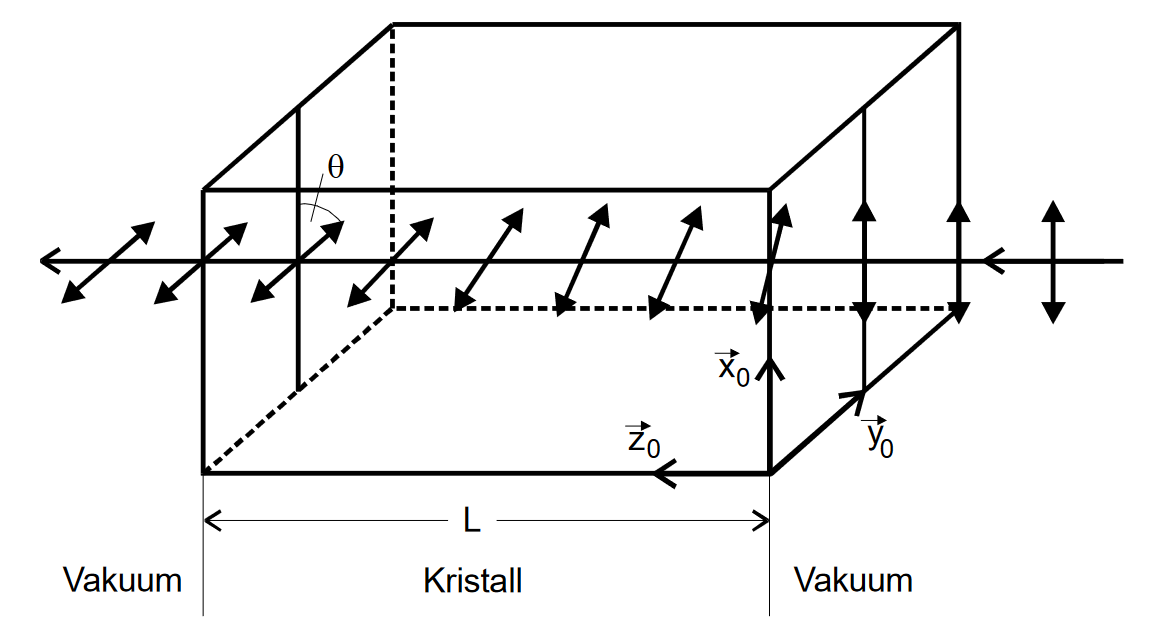
\includegraphics[width=\textwidth]{Bilder/faradayeffekt.png}
    \caption{Schematischer Verlauf eines polarisierten Lichtstrahls durch ein Medium, das die Polarisation ändert. Das Magnetfeld liegt parallel zur Ausbreitungsrichtung des Lichtstrahls. \cite{anhang}}
    \label{fig:faradayeffekt}
\end{figure}
Beim Faraday-Effekt wird linear polarisiertes Licht über zwei verschiedene zirkular polarisierte Anteile beschrieben. Diese beiden Anteile führen dazu, dass sich Elektronen im zu untersuchenden Medium auf zirkularen Bahnen bewegen, was dazu führt, dass diese ein Magnetfeld ausbilden.
Dieses kann einem parallel zur Ausbreitungsrichtung des Lichtes stehenden Magnetfeld entgegenwirken oder mitwirken. Diese Interaktion führt dazu, dass sich ein Phasenunterschied zwischen den beiden zirkularen Anteilen ausbildet,
was schlussendlich dazuführt, dass die ursprüngliche Polarisation des Lichtes sich ändert, bspws. kann parallel polarisiertes Licht nun senkrecht polarisiert sein. \\
Wirkt diese Änderung auch ohne das Wirken eines äußeren Magnetfeldes, wird von optischer Aktivität gesprochen. \\
Der Rotationswinkel des polarisierten Lichtes beim Faraday-Effekt hängt von der Stärke des Magnetfeldes und der durchlaufenen Distanz ab,

\begin{equation*}
    \theta = V \cdot B \cdot L 
    \label{eq:verdet}
\end{equation*}

wobei $B$ das Magnetfeld, $L$ die durchdringte Distanz und $V$ die Verdet-Konstante ist, die material- und frequenzabhängig ist. \cite{heintze}
Es kann nun gezeigt werden \cite{anhang}, dass für die Poleraisation des Winkels weiter
\begin{equation*}
    \theta(\lambda) = \frac{2 \pi^2 e_0^3 c}{\epsilon_0} \frac{1}{m^2} \frac{1}{\lambda^2 \omega_0^2} \frac{NBL}{n}
    \label{eq:theta_ohne_effektivemasse}
\end{equation*}
gilt, wobei $e_0$ die Elementarladung, $c$ die Lichtgeschwindigkeit, $\epsilon_0$ die elektrische Permittivität, $\lambda$ die Wellenlänge, $\omega_0$ die Resonanzfrequenz des Halbleiters, $m$ die Masse der Elektronen, $N$ die Dopant-Konzentration, $B$ die magnetische
Flussdichte, $L$ die vom Licht durchdringte Länge und $n$ der Brechungsindex im Material zu $\lambda$ ist.\\
Führt man die Faraday-Rotation pro Längeneinheit $\theta_\text{frei} = \frac{\theta}{L}$ ein und setzt die effektive Masse $m^{*}$ ein, ergibt sich
\begin{equation}
    \theta_\text{frei} = \frac{e_0^3}{8 \pi^2 \epsilon_0 c^2} \cdot \frac{\lambda^2}{(m^{*})^2} \cdot \frac{NB}{n}. 
    \label{eq:theta_frei}
\end{equation}
\cite{anhang}